%%%%%%%%%%%%%%%%%%%%%%%%%%%%%%%%%%%%%%%%%
% University/School Laboratory Report
% LaTeX Template
% Version 4.0 (March 21, 2022)
%
% This template originates from:
% https://www.LaTeXTemplates.com
%
% Authors:
% Vel (vel@latextemplates.com)
% Linux and Unix Users Group at Virginia Tech Wiki
%
% License:
% CC BY-NC-SA 4.0 (https://creativecommons.org/licenses/by-nc-sa/4.0/)
%
%%%%%%%%%%%%%%%%%%%%%%%%%%%%%%%%%%%%%%%%%

%----------------------------------------------------------------------------------------
%	PACKAGES AND DOCUMENT CONFIGURATIONS
%----------------------------------------------------------------------------------------

\documentclass[
	letterpaper, % Paper size, specify a4paper (A4) or letterpaper (US letter)
	10pt, % Default font size, specify 10pt, 11pt or 12pt
]{CSUniSchoolLabReport}

%packages
\usepackage{minted}
\usepackage{import}

\addbibresource{sample.bib} % Bibliography file (located in the same folder as the template)

%----------------------------------------------------------------------------------------
%	REPORT INFORMATION
%----------------------------------------------------------------------------------------

\title{Building an Integer ALU Step 2\\ CS 3339 \\ Group: The Architects} % Report title

\author{Aaron \textsc{Reed} \& Carlo \textsc{Marroquin} \& Ryan \textsc{Bieker}} % Author name(s), add additional authors like: '\& James \textsc{Smith}'

\date{\today} % Date of the report

%----------------------------------------------------------------------------------------

\begin{document}

\maketitle % Insert the title, author and date using the information specified above

\begin{center}
	\begin{tabular}{l r}
		Instructor: & Professor \textsc{Klepetko} % Instructor/supervisor
	\end{tabular}
\end{center}

%----------------------------------------------------------------------------------------
%	OBJECTIVE
%----------------------------------------------------------------------------------------

\section{Objective}

To introduce the process and methodology of designing a new computer circuit from scratch by coding 4-bit Binary Functions And, Nand, Or, Nor, Xor, Xnor, Not, and a Shifter. 4-bit arithmetic operations Addition, Subtraction, Multiplication all including carry in and carry out circuits 

\section{Verilog Code}
%AND verilog
\section{AND Design}
\begin{center}
    \inputminted{octave}{verilog/and_4b/and_4b.v}
\end{center}
\section{AND Testbench}
\begin{center}
    \inputminted{octave}{verilog/and_4b/and_4b_test.v}
\end{center}

%NAND verilog
\section{NAND Design}
\begin{center}
    \inputminted{octave}{verilog/nand_4b/nand_4b.v}
\end{center}
\section{NAND Testbench}
\begin{center}
    \inputminted{octave}{verilog/nand_4b/nand_4b_test.v}
\end{center}

%OR verilog
\section{OR Design}
\begin{center}
    \inputminted{octave}{verilog/or_4b/or_4b.v} %insert design file here
\end{center}
\section{OR Testbench}
\begin{center}
    \inputminted{octave}{verilog/or_4b/or_4b_test.v} %insert testbench file here
\end{center}

%NOR verilog
\section{NOR Design}
\begin{center}
    \inputminted{octave}{verilog/nor_4b/nor_4b.v} %insert design file here
\end{center}
\section{NOR Testbench}
\begin{center}
    \inputminted{octave}{verilog/nor_4b/nor_4b_test.v} %insert testbench file here
\end{center}

%XOR verilog
\section{XOR Design}
\begin{center}
    \inputminted{octave}{verilog/xor_4b/xor_4b.v} %insert design file here
\end{center}
\section{XOR Testbench}
\begin{center}
    \inputminted{octave}{verilog/xor_4b/xor_4b_test.v} %insert testbench file here
\end{center}

%XNOR verilog
\section{XNOR Design}
\begin{center}
    \inputminted{octave}{verilog/xnor_4b/xnor_4b.v} %insert design file here
\end{center}
\section{XNOR Testbench}
\begin{center}
    \inputminted{octave}{verilog/xnor_4b/xnor_4b_test.v} %insert testbench file here
\end{center}

%NOT verilog
\section{NOT Design}
\begin{center}
    \inputminted{octave}{verilog/not_4b/not_4b.v} %insert design file here
\end{center}
\section{NOT Testbench}
\begin{center}
    \inputminted{octave}{verilog/not_4b/not_4b_test.v} %insert testbench file here
\end{center}

%SHIFT verilog
\section{SHIFT Design}
\begin{center}
    \inputminted{octave}{verilog/shift_4b/shift_4b.v} %insert design file here
\end{center}
\section{SHIFT Testbench}
\begin{center}
    \inputminted{octave}{verilog/shift_4b/shift_4b_test.v} %insert testbench file here
\end{center}

%ADDITION verilog
\section{ADDITION Design}
\begin{center}
    \inputminted{octave}{verilog/add_4b/add_4b.v} %insert design file here
\end{center}
\section{ADDITION Testbench}
\begin{center}
    \inputminted{octave}{verilog/add_4b/add_4b_test.v} %insert testbench file here
\end{center}

%SUBTRACTION verilog
\section{SUBTRACTION Design}
\begin{center}
    \inputminted{octave}{verilog/sub_4b/sub_4b.v} %insert design file here
\end{center}
\section{SUBTRACTION Testbench}
\begin{center}
    \inputminted{octave}{verilog/sub_4b/sub_4b_test.v} %insert testbench file here
\end{center}

%MULTIPLICATION verilog
\section{MULTIPLICATION Design}
\begin{center}
    \inputminted{octave}{verilog/mult_4b/mult_4b.v} %insert design file here
\end{center}
\section{MULTIPLICATION Testbench}
\begin{center}
    \inputminted{octave}{verilog/mult_4b/mult_4b_test.v} %insert testbench file here
\end{center}

\section{Waveforms}
\section{AND}
The AND function took only 4 bit inputs X and Y then used them in a logical AND function.

%\begin{tabular}{l l}
	%The NAND gate is NOT and. So we took two 1-bit integers to preform an and operation before doing the logical NOT operation. %& \SI{7.28}{\gram}\\ % Scientific/technical units are output using the \SI command, see the siunitx package documentation for more information on how to use this command
	%Mass of crucible and magnesium before heating & \SI{8.59}{\gram}\\
	%Mass of crucible and magnesium oxide after heating & \SI{9.46}{\gram}\\
	%Balance used & \#4\\
	%Magnesium from sample bottle & \#1
%\end{tabular}
\begin{figure}[H] % [H] forces the figure to be placed exactly where it appears in the text
	%\centering % Horizontally center the figure
	\includegraphics[width=1.2\textwidth]{Figures Part2/image.png} % Include the figure
	\caption{The AND function's waveform.}
\end{figure}
%----------------------------------------------------------------------------------------
%	SAMPLE CALCULATION
%----------------------------------------------------------------------------------------

\section{NAND}
The NAND function took 4 bit inputs X and Y as well, then preformed the logical NAND. An out is displayed on our waveform.

\begin{figure}[H] % [H] forces the figure to be placed exactly where it appears in the text
	%\centering % Horizontally center the figure
	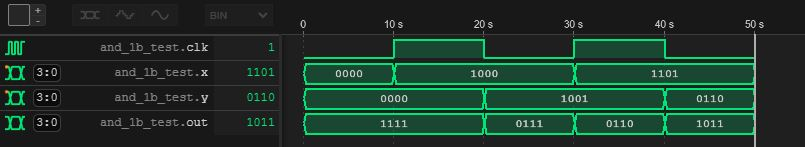
\includegraphics[width=1.2\textwidth]{Figures Part2/nand_4b_figure.JPG} % Include the figure
	\caption{The NAND function's waveform.}
\end{figure}

%----------------------------------------------------------------------------------------
%	RESULTS AND CONCLUSIONS
%----------------------------------------------------------------------------------------

\section{OR}
The OR function took inputs x and y, each 4 bits. Out is also displayed on the waveform. Then it preformed the logical OR on both 4 bit numbers.

\begin{figure}[H] % [H] forces the figure to be placed exactly where it appears in the text
	%\centering % Horizontally center the figure
	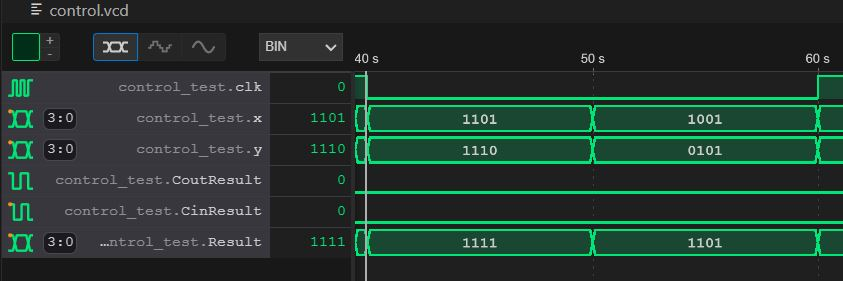
\includegraphics[width=1.2\textwidth]{Figures Part2/or.png} % Include the figure
	\caption{The OR functions waveform.}
\end{figure}

%----------------------------------------------------------------------------------------
%	DISCUSSION
%----------------------------------------------------------------------------------------

\section{NOR}
The NOR function took the 4 bit inputs X and Y, out is displayed on the waveform. Then the logical NOR was preformed and waveform produced.

\begin{figure}[H] % [H] forces the figure to be placed exactly where it appears in the text
	%\centering % Horizontally center the figure
	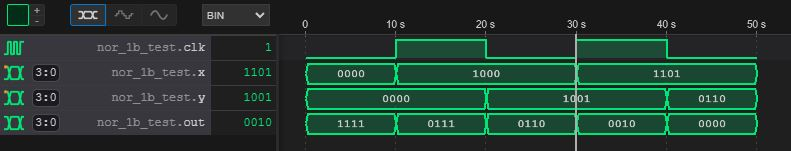
\includegraphics[width=1.2\textwidth]{Figures Part2/nor_4b_figure.JPG} % Include the figure
	\caption{The NOR function Waveform.}
\end{figure}

%----------------------------------------------------------------------------------------
%	ANSWERS TO DEFINITIONS
%----------------------------------------------------------------------------------------

\section{XOR}
The XOR function took two 4 bit inputs X and Y. Then the logical XOR is preformed, an out is also displayed on the waveform.

\begin{figure}[H] % [H] forces the figure to be placed exactly where it appears in the text
	%\centering % Horizontally center the figure
	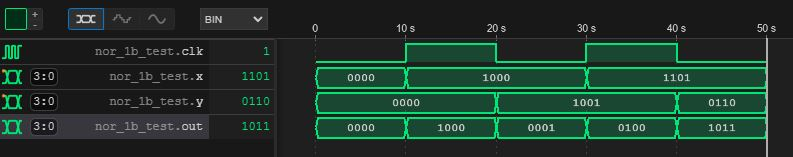
\includegraphics[width=1.2\textwidth]{Figures Part2/xor_4b_figure.JPG} % Include the figure
	\caption{The XOR waveform.}
\end{figure}



\section{XNOR}
The XNOR function receives two 4-bit inputs X and Y. When the individual bits are the same, the output bit-place is 1.

\begin{figure}[H] % [H] forces the figure to be placed exactly where it appears in the text
	%\centering % Horizontally center the figure
	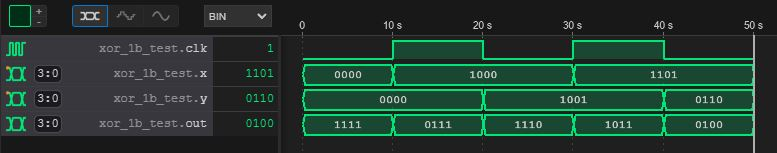
\includegraphics[width=1.2\textwidth]{Figures Part2/xnor_4b_figure.JPG} % Include the figure
	\caption{The XNOR wave form.}
\end{figure}


\section{NOT}
The NOT module receives one 4-bit input and flips the value of each bit. 

\begin{figure}[H] % [H] forces the figure to be placed exactly where it appears in the text
	%\centering % Horizontally center the figure
	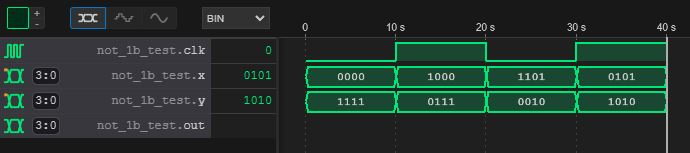
\includegraphics[width=1.2\textwidth]{Figures Part2/not_4b_figure.JPG} % Include the figure
	\caption{The 4-bit NOT waveform.}
\end{figure}


\section{SHIFT}
The SHIFT module receives one 4-bit input and shifts the bits right or left and. 

\begin{figure}[H] % [H] forces the figure to be placed exactly where it appears in the text
	%\centering % Horizontally center the figure
	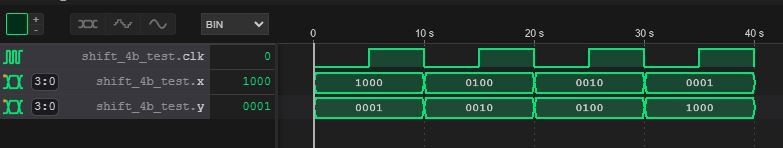
\includegraphics[width=1.2\textwidth]{Figures Part2/shift_4b_figure.JPG} % Include the figure
	\caption{The 4-bit SHIFT waveform.}
\end{figure}


\section{ADDITION}
The ADD module receives two 4-bit inputs and adds the two values together. If the value exceeds 4-bits a Carry-out is assigned to 1.

\begin{figure}[H] % [H] forces the figure to be placed exactly where it appears in the text
	%\centering % Horizontally center the figure
	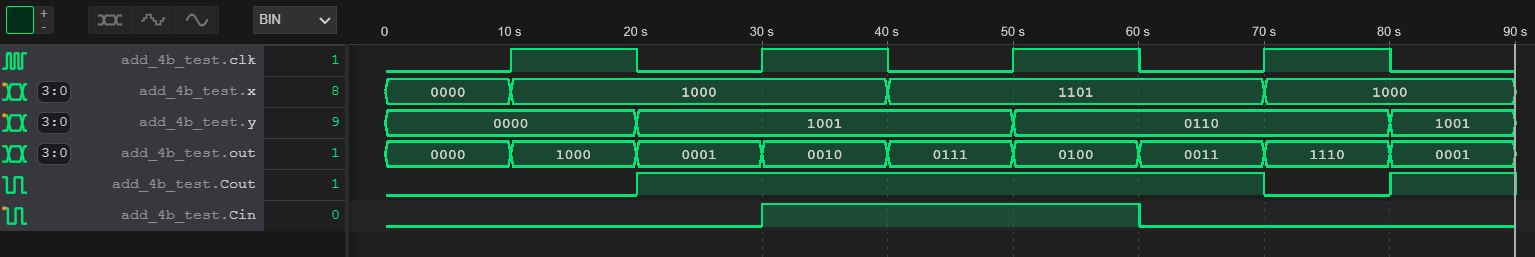
\includegraphics[width=1.2\textwidth]{Figures Part2/add_4b_figure.png} % Include the figure
	\caption{The 4-bit ADDITION waveform.}
\end{figure}

\section{SUBTRACTION}
The SUBTRACTION module receives two 4-bit inputs and subtracts the second 4-bit value from the first with an output using two's complement. 

\begin{figure}[H] % [H] forces the figure to be placed exactly where it appears in the text
	%\centering % Horizontally center the figure
	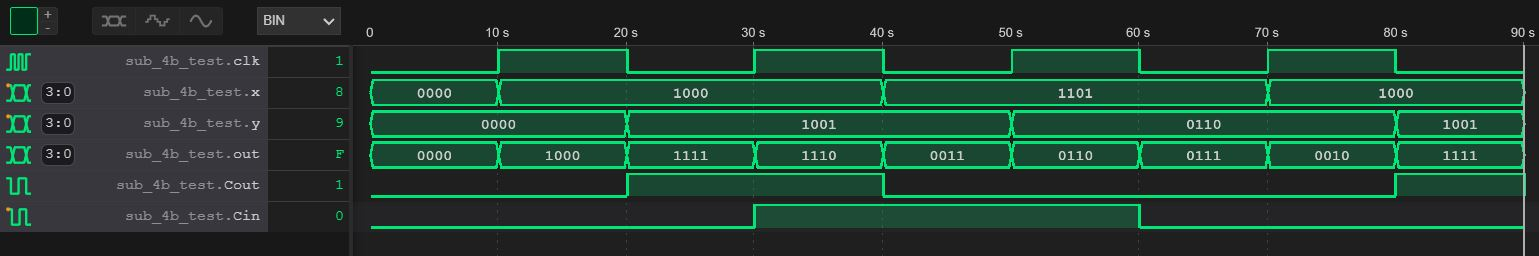
\includegraphics[width=1.2\textwidth]{Figures Part2/sub_4b_figure.JPG} % Include the figure
	\caption{The 4-bit SUBTRACTION waveform.}
\end{figure}


\section{MULTIPLICATION}
The MULTIPLICATION module receives two 4-bit values, multiplies the two together, and produces an 8-bit output. 

\begin{figure}[H] % [H] forces the figure to be placed exactly where it appears in the text
	%\centering % Horizontally center the figure
	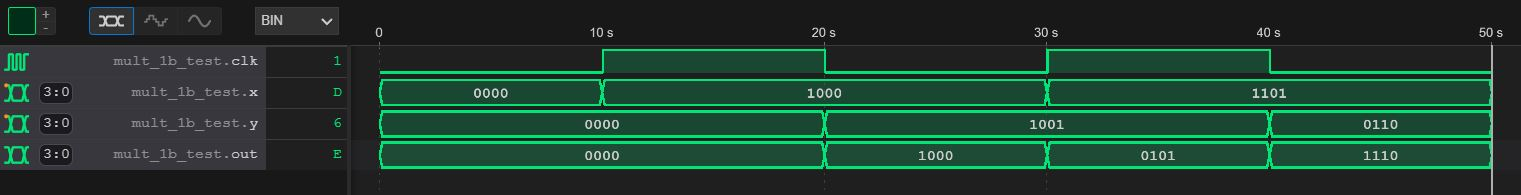
\includegraphics[width=1.2\textwidth]{Figures Part2/mult_4b_figure.JPG} % Include the figure
	\caption{The 4-bit MULTIPLICATION waveform.}
\end{figure}

%\section{Answers to Definitions}

%\begin{enumerate}
%	\item The \textit{atomic weight of an element} is the relative weight of one of its atoms compared to C-12 with a weight of 12.0000000$\ldots$, hydrogen with a weight of 1.008, to oxygen with a weight of 16.00. Atomic weight is also the average weight of all the atoms of that element as they occur in nature.
%	\item The \textit{units of atomic weight} are two-fold, with an identical numerical value. They are g/mole of atoms (or just g/mol) or amu/atom.
%	\item \textit{Percentage discrepancy} between an accepted (literature) value and an experimental value is:
%		\begin{equation*}
%			\frac{\mathrm{experimental\;result} - \mathrm{accepted\;result}}{\mathrm{accepted\;result}}
%		\end{equation*}
%\end{enumerate}

%----------------------------------------------------------------------------------------
%	BIBLIOGRAPHY
%----------------------------------------------------------------------------------------
\section{Conclusion}
In order to create our 4-bit modules in Verilog, we had to determine how to store 4-bit numbers in registers and wires. Addition was the most straightforward to code with Carry-In and Carry-Out values.  In our multiplication module, we found that the product of two 4-bit numbers needed to be 8-bits in order to properly implement the Carry-Out of the module. The multiplication module gave us the most trouble as we couldn’t decide what size the output product should be. The logic gates were quick to get through using 4-bit values as they are built into the Verilog code as operators.

%\printbibliography % Output the bibliography

%----------------------------------------------------------------------------------------

\end{document}
